\documentclass{article}
\usepackage[utf8]{inputenc}
\usepackage{natbib}
\usepackage{graphicx}
\usepackage{lastpage}
\usepackage{xcolor}
\usepackage{lipsum}
\usepackage[T1]{fontenc}
\usepackage{fancyhdr}
\usepackage{geometry}
\usepackage{url}
\usepackage[dutch]{babel}


\usepackage{color}
\usepackage{pdfpages} %om pdf files met requirements lijsten toe te voegen




\bibliographystyle{abbrv} %abbrvnat geeft problemen

\title{Software Requirements Specification}
\author{} %leave empty
\date{19 november 2014} %ok, manuele datum

\addtolength{\footskip}{1.3cm} % make more space for the footer
\pagestyle{fancyplain} % use fancy for all pages except chapter start
\lhead{}
\cfoot{
\includegraphics[height=1.3cm]{Small_Logo.png}} % right logo
\rfoot{\thepage}
\renewcommand{\headrulewidth}{0.3pt} % remove rule below header
\renewcommand{\footrulewidth}{0.3pt} % remove rule below header

\begin{document}

\makeatletter
\begin{titlepage}

\newcommand{\HRule}{\rule{\linewidth}{0.7mm}} % Defines a new command for the horizontal lines, change thickness here


\vspace*{1.2mm}

\center 

\includegraphics[scale=0.6]{Logo.png}\\[1cm] 
%---------------------------------------------------------------------------------------
%	HEADINGS SECTION
%----------------------------------------------------------------------------------------

\textsc{\LARGE Vrije Universiteit Brussel}\\[0.3cm] % Name of your university/college
\textsc{\large WE-DINF-6537}\\
\textsc{\large Project Software Engineering}\\
\textsc{\large Academiejaar 2014-2015}\\[0.3cm] 
%\textsc{\large Software Engineering}\\[0.7cm] % Major heading such as course name

%----------------------------------------------------------------------------------------
%	TITLE SECTION
%----------------------------------------------------------------------------------------

\HRule \\[0.4cm]
{ \huge \bfseries \@title \\[0.5cm] }
\HRule \\[0.5cm]
 
%----------------------------------------------------------------------------------------
%	AUTHOR SECTION
%----------------------------------------------------------------------------------------

\Large
% laat voorlopig nog even de namen/mailadressen op deze pagina staan
% eerst moeten we zien of er een beter alternatief is om de lege plek dan op te vullen
% anders laten we ze gewoon staan...

%volgens mij ziet het er zo heel goed uit, maar als ze echt wegmoeten mss vub logo groter maken? 
% => OK, ik vind het ook veter zo, we laten ze staan!
Douglas Horemans \textit{<dhoreman@vub.ac.be>}\\
Hannah Pinson \textit{<hpinson@vub.ac.be>}\\
Ivo Vervlimmeren \textit{<ivervlim@vub.ac.be>}\\
Noah Van Es \textit{<noahves@vub.ac.be>}\\
Pieter Steyaert \textit{<psteyaer@vub.ac.be>}\\

\vspace{0.6cm}


\includegraphics[scale=0.4]{VUB_schild.pdf}\\[0.5cm]

{\large 19 november 2014}
\vfill % Fill the rest of the page with whitespace

\end{titlepage}

\newpage
\section*{Versiegeschiedenis}
\addcontentsline{toc}{section}{Versiegeschiedenis}

\begin{center}
\begin{tabular}[t]{| c | c | c | c |}
    \hline
    \textbf{Versie} & \textbf{Datum} & \textbf{Auteurs\cite{note:author}} & \textbf{Beschrijving} \\
    \hline
    
    1.0     &  19/11/2014   &   \begin{tabular}{c} 
                                    Douglas Horemans \\
                                \end{tabular} & Eerste versie \\
    \hline
    2.0     &  15/12/2014   &   \begin{tabular}{c} 
                                    Douglas Horemans \\
                                \end{tabular} & tweede versie \\
    \hline
\end{tabular}
\end{center}
\newpage



\tableofcontents
\newpage

%%%%%%%%%%%%%%%%%%%%%%%%%%%%%%%%%% INTRODUCTIE

\section{Introductie}

%%%
\subsection{Doel en doelpubliek} %van het SRS, niet van het project
Dit is het Software Requirements Specification (SRS) document voor SKRIBL,  een softwareproject uitgevoerd door de groep SE4\_1415 in het kader van het opleidingsonderdeel Software Engineering van de Vrije Universiteit Brussel. Dit document is opgesteld volgens de IEEE 1016-2009 standaard. \newline
\\
\noindent De algemene eisen die de klant aan het op te leveren product stelt zijn te vinden in de projectomschrijving van het opleidingsonderdeel \cite{Xtreport:organisatie}. Dit SRS biedt een globaal, gestructureerd overzicht van deze vereisten (user requirements) in onderdeel (\ref{subsec:userRequirements}). Daarnaast is er een gedetailleerde oplijsting van system requirements die voortvloeien uit deze user requirements, en die dienen als richtlijnen bij het ontwikkelen en testen van het softwareproduct, in onderdeel (\ref{sec:systemRequirements}). In overeenstemming met de principes van een agile development proces worden de system requirements in dit SRS \emph{bij iedere sprint} aangevuld. Meer informatie over het doel en de planning van deze sprints is te vinden in het Software Project Management Plan \cite{Xtreport:SPMP}. \newline
\\
\noindent Dit document is zowel bedoeld voor de klant en externe controle als voor de interne organisatie. In het bijzonder worden de system requirements in onderdeel (\ref{sec:systemRequirements}) door alle leden van het team gebruikt als richtlijnen bij het volledige plannings-, ontwikkelings- en testproces van iedere sprint. De globale oplijsting van requirements in onderdeel (\ref{subsec:userRequirements}) dient als handvest voor de grote lijnen van het software design en de algemene planning van het project.  

%%%
\subsection{Product Scope}
Het doel van dit softwareproject is het ontwikkelen van SKRIBL, een webapplicatie die het enerzijds mogelijk maakt voor onderzoekers om wetenschappelijke publicaties te beheren en die anderzijds de netwerken van deze onderzoekers analyseert en op een aantrekkelijke manier visualiseert. Deze applicatie wordt binnen het kader van het opleidingsonderdeel software engineering gecre\"{e}erd gedurende het academiejaar 2014-2015.

%%%
\subsection{Gebruikte conventies en afkortingen}
Suggesties en opmerkingen voor toekomstige aanpassingen in dit document worden aangeduid met vierkante haakjes en een cursief lettertype: [{\it voorbeeld suggestie}]. \newline
\\
\noindent Volgende afkortingen worden in dit SRS gebruikt:
\begin{itemize}
\item SRS: Software Requirements Specification (document)
\item SPMP: Software Project Management Plan (document)
%\item STD:  Software Test Plan (document)
%\item SDD: Software Design Document (document)
\item FR-U: Functional Requirement, type User
\item FR-P: Functional Requirement, type Publicatie
\item FR-D: Functional Requirement, type Data-Mining
\item NFR-S: Niet-Functionele Requirement, type Security
\item NFR-R: Niet-Functionele Requirement, type Reliability
\item NFR-P: Niet-Functionele Requirement, type Performance
\item NG: Nieuwe Gebruiker
\end{itemize}


%%%
\subsection{Referenties}
\begingroup
\renewcommand{\section}[2]{}% verwijdert titel sectie referenties
\bibliography{referenties}
\endgroup

\clearpage
%%%%%%%%%%%%%%%%%%%%%%%%%%%%%%%%%% ALGEMENE BESCHRIJVING 

\section{Algemene Beschrijving}

\subsection{Perspectief van het product}
De ontwikkelde webapplicatie is een op zichzelf staand softwareproduct. Het maakt geen deel uit van andere softwareproducten maar steunt voor een deel van zijn content (i.e., aangeleverde publicaties) op het contacteren van andere websites met gelijkaardige functionaliteiten. \newline
\\
%----comment----%
\noindent [{\it Volgens de IEEE standaard moeten in de onderdeel verder nog de interfaces (System interfaces; User interfaces; Hardware interfaces; Software interfaces;Communications interfaces) beschreven worden. Indien van toepassing zullen deze onderdelen, in samenspraak met de Software Architect en Configuration Manager, in latere versies aangevuld worden.}]

\subsection{Functies van het product}
\label{subsec:userRequirements}

Hieronder volgt een gestructureerde oplijsting van de functionele vereisten zoals beschreven in de projectomschrijving van het opleidingsonderdeel \cite{Xtreport:organisatie}.

\renewcommand{\labelitemi}{$\diamond$}
\renewcommand{\labelitemii}{$\bullet$}
\renewcommand{\labelitemiii}{$\cdot$}

\begin{itemize}
    %%
    %USER %
    %%
    \item USER
    \begin{itemize}
        \item inloggen en uitloggen 
        \item account aanmaken
        \item account beheren 
        \item aanleggen en beheren van portfolio eigen publicaties
        \item persoonlijke score via portfolio
	\item toevoegen en beheren van lijst publicaties van derden ("favorieten")
	\item publicaties opslaan op eigen computer, buiten applicatie
	\item top drie relevantste publicaties binnen onderzoeksdomein 
	\item suggesties van relevante papers en feed-back/voorkeuren 
	\item opzoeken en toevoegen van publicaties, gevonden in systeem en/of internet, via invulformulier of reeds toegevoegde publicaties
	\item annoteren van publicaties, toevoegen van bijlagen 
	\item publicaties linken op manieren die systeem niet standaard voorziet
	\item raadplegen, genereren en exporteren (PDF) van persoonlijk statistieken en bijhorende grafieken
	\item visualisatie van en interactie met sociaal netwerk in een graaf
	\item mobiele interface
    \end{itemize}
   %%
    %PUBLICATIES %
    %%
    \item PUBLICATIES 
    \begin{itemize}
    \item toevoegen van content + metadata door extractie uit PDF/BibTex en/of manuele aanvulling
    \item weergave van publicaties 
    \item downloaden van het internet
    \item opslaan op computer vd gebruiker (buiten applicatie)
    \end{itemize}
     %%
    %DATAMINING %
    %%
    \item DATAMINING 
    \begin{itemize}
    \item persoonlijke score van gebruiker berekenen adhv portfolio: 
    	\begin{itemize}
    		\item aantal eigen publicaties gedeeld door het aantal maanden sinds de eerste publicatie
   		 \item kwaliteit op basis van de classificatie van conferences en journals
    		\item impact van de eigen publicatie (aantal citaties)
    	\end{itemize}
    \item relevantie van publicatie voor gebruiker berekenen in functie van onderzoeksdomein 
    \item relevantie van publicatie voor gebruiker berekenen op basis van co-auteurs, keywords, ... en dynamische voorkeuren gebruiker 
    \item statistieken voor gebruiker berekenen adhv volgende metrieken (zie ook persoonlijke score)
      	\begin{itemize}
    		\item publicaties per jaar
   		 \item ranking van de publicaties (afhankelijk van de ranking van conference/journal)
    		\item aantal citaties
    	\end{itemize}
    \end{itemize}
\end{itemize}




\subsection{Gebruikers}
De beoogde gebruikers zijn onderzoekers actief in de wetenschappelijke wereld. Deze vormen de enige klasse van gerechtmatigde gebruikers. Daarnaast worden er verschillende veiligheidsmaatregelen ingebouwd om niet-rechtmatige gebruikers de toegang tot de applicatie te ontzeggen. 

\subsection{Omgeving}
Aan de back-end draait het systeem op Wilma, een server beschikbaar gesteld aan de studenten wetenschappen van de Vrije Universiteit Brussel.  Front-end ondersteunt de applicatie alle gangbare en up-to-date browsers. De mobiele interface wordt ontwikkeld voor Android smartphones.

\subsection{Beperkingen op design en implementatie}
JavaScript, HTML5, CSS en bijbehorende open-source frameworks en bibliotheken zijn de enige programmeertalen en technologie\"{e}n die gebruikt mogen worden. In het algemeen mag enkel vrije software aangewend worden, en deze software moet ook verantwoord kunnen worden. Er moet daarnaast ten allen tijde gebruik worden gemaakt van een testing framework. Code moet volgens een vooraf vastgelegde standaard voorzien worden van commentaar. Ten slotte moet GitHub gebruikt worden als (publieke) repository. 

\subsection{Gebruikshandleidingen}

[{\it nog te bepalen}]




\clearpage
%%%%%%%%%%%%%%%%%%%%%%%%%%%%%%%%%% SYSTEEM REQUIREMENTS
\section{Specifieke Requirements}
\label{sec:systemRequirements}


\subsection{Functionele Requirements}
\noindent De functionele requirements zijn opgedeeld in drie types: gebruikers (FR-U), publicaties (FR-P) en data-mining (FR-D). Verder worden ze gegroepeerd volgens feature. De prioriteiten worden aangegeven met kleuren: Rood = hoge prioriteit, Oranje = gemiddelde prioriteit, Groen = lage prioriteit. De specifieke requirements worden weergegeven op de volgende pagina's.

\subsection{Niet-Functionele Requirements}
\noindent De functionele requirements zijn opgedeeld in drie types: reliability (NFR-R), performance (NFR-P) en security (NFR-S). Ze  worden gegroepeerd volgens deze types. De prioriteiten worden aangegeven met kleuren: Rood = hoge prioriteit, Oranje = gemiddelde prioriteit, Groen = lage prioriteit. De specifieke requirements worden weergegeven op de volgende pagina's.

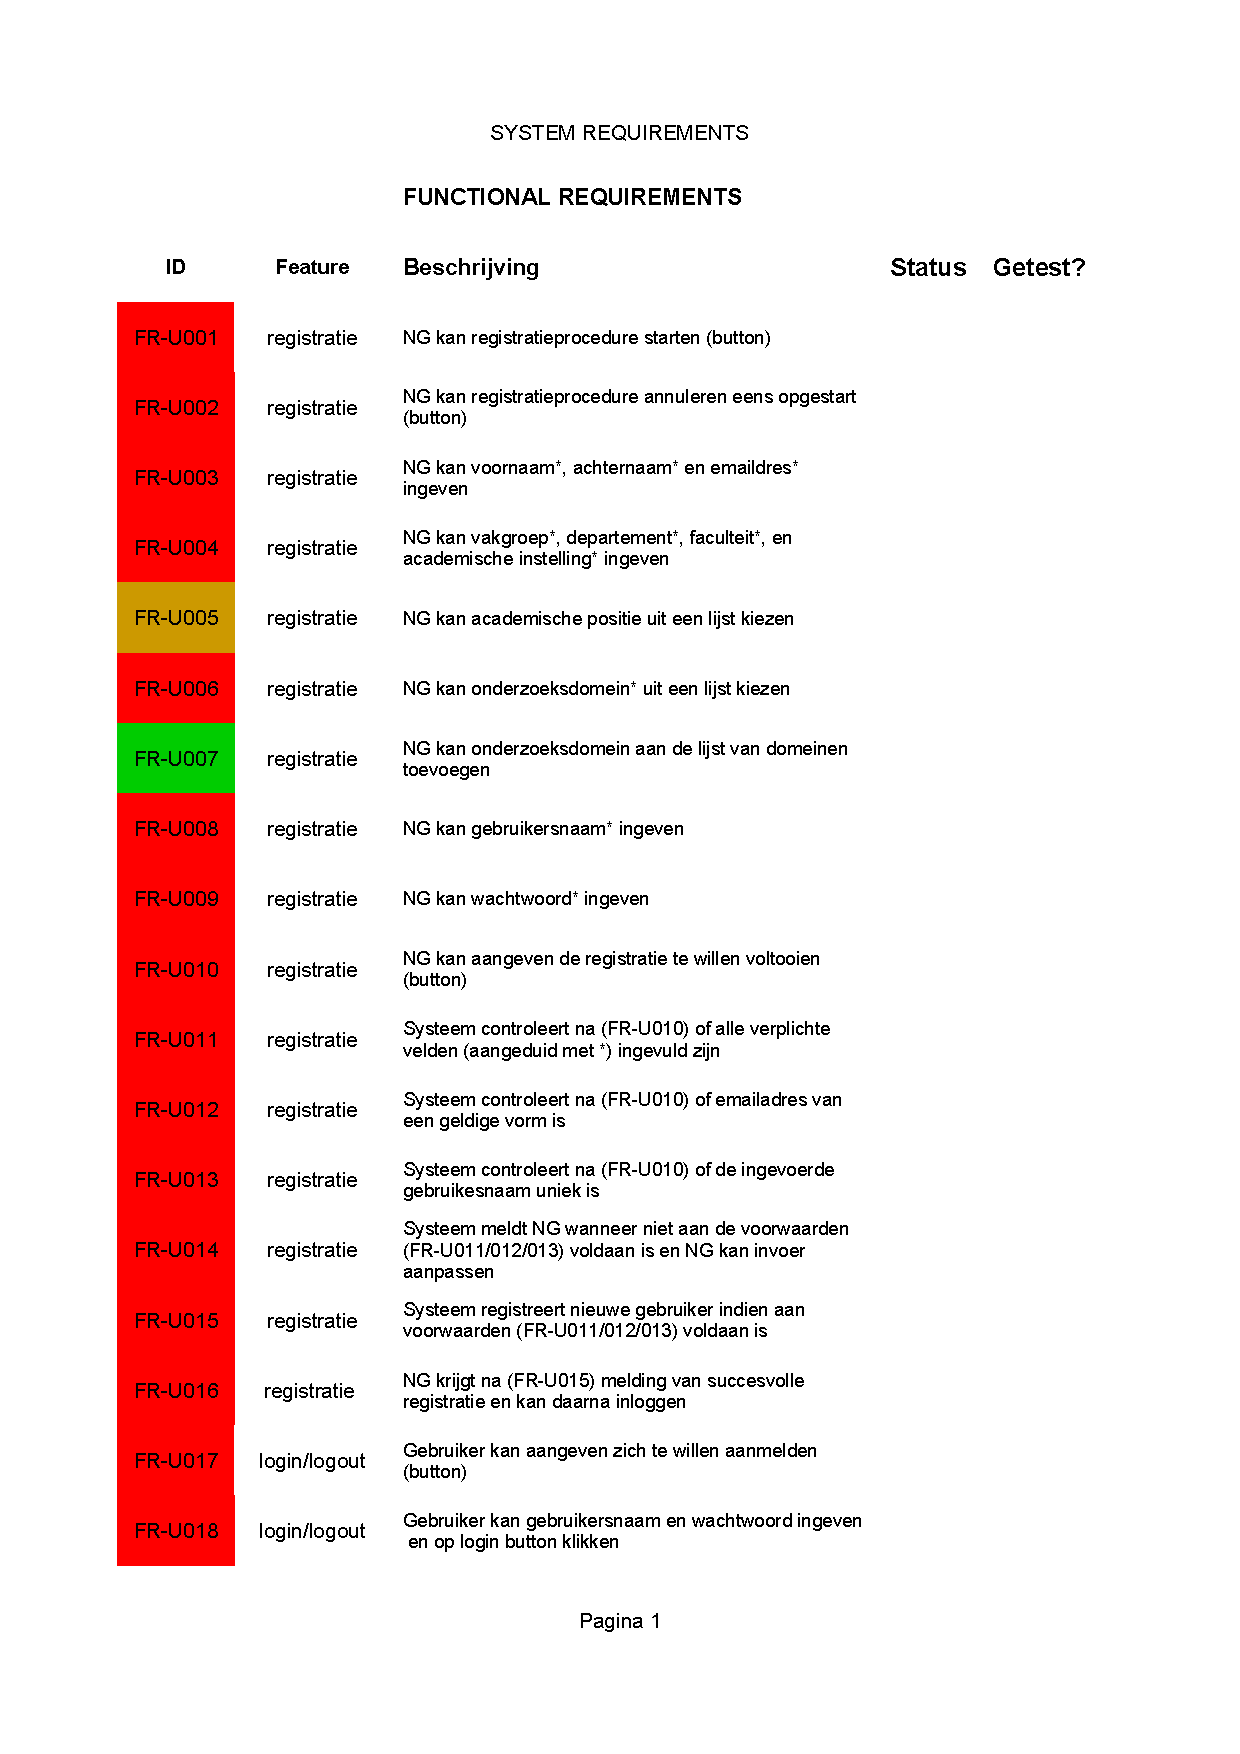
\includepdf[pages={-}]{reqList_sprint1.pdf}








\end{document}
